Para comenzar con las pruebas lo primero que se realizó es la conexión de diversos sensores en una protoboard. Se generó un programa de Arduino dónde a través de I2C se realizaba la comunicación. \\ Conjuntamente con estos sensores de Presión, Humedad y Temperatura se utilizó un sensor para medir presión diferencial, para digitalizar estos datos valores se utilizó un convertidor analógico digital.

\paragraph*{Elementos utilizados}
		\begin{itemize}
			\item  \textbf{BME280:} Sensor de presión atmosférica, temperatura y humedad relativa.
			\item \textbf{SI7021:} Sensor de temperatura y humedad relativa.
			\item \textbf{MPX7002:} Sensor de presión diferencial.
			\item \textbf{ADS1115:} Convertidor analógico digital 16bits.
		\end{itemize}

\begin{figure}[htb]
	\centering
	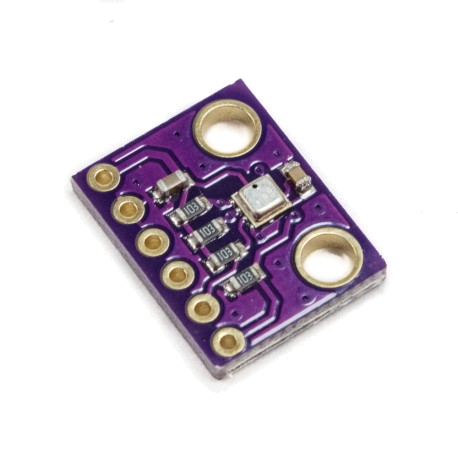
\includegraphics[scale=0.35]{bme280.png}
	\caption{figure}{BME280}
	\label{fig:BME280}
\end{figure}

	

    \subsection{Programa Arduino}
        \subsubsection{Ecuación velocidad del aire}
	%	densidad_funcion_P_T_H.pdf  dentro del drive
    \subsection{Pruebas}
    aca explicar que se hizo sin filtros y porq se filtro despues
        \subsubsection{Filtros}
        que filtro se utilizo y porq y cuando
    - Poner donde se agrego.

\newpage